\section{Temperature and Ideal Gases}
\subsection{Thermal Equilibrium}
\vocab{Temperature}: a measure of degree of hotness of an object. Thermal energy moves from object at higher temperature to object at lower temperature.

\begin{remark}
Temperature does not measure amount of thermal energy; it only indicates direction of heat flow.
\end{remark}

\vocab{Heat}: (thermal) energy that flows from region of higher to lower temperature\footnote{through conduction, convection and radiation.}. 

\begin{defn}{Thermal equilibrium}{}
When two objects in thermal contact are in thermal equilibrium, there is no \emph{net} heat transfer between them. They are at the same temperature.
\end{defn}

\begin{defn}{Zeroth law of Thermodynamics}{}
If objects $A$ and $B$ are separately in thermal equilibrium with a third object $C$, then $A$ and $B$ are also in thermal equilibrium with each other.
\end{defn}

\begin{remark}
Object $C$ can function as a thermometer to determine if temperatures of two objects are the same. This allows us to determine whether temperatures of two objects are same, without both objects being in contact.
\end{remark}
\pagebreak

\subsection{Temperature Scales}
\subsubsection{Empirical Scale}
\vocab{Empirical temperature scale}: scale of temperature based on variation of some physical property with temperature.
\begin{enumerate}
\item Choose appropriate thermometric property

Thermometric property varies \textbf{linearly} with temperature. Some examples include: 
    \begin{itemize}
    \item volume of fixed mass of liquid (liquid-in-glass thermometer)
    \item resistance of metal (platinum resistance thermometer)
    \item pressure of fixed mass of gas at constant volume (constant volume gas thermometer)
    \item e.m.f. produced between junctions of dissimilar metals at different temperatures (thermocouple thermometer)
    \end{itemize}

\item Select two fixed points

Usually \textbf{ice point} of water (0 \degree C) and \textbf{steam point} of water (100 \degree C).

\item Calibrate thermometer

Place it in systems of lower and upper fixed points. Record values of thermometric quantity. Assume linear relationship between these two points.
\end{enumerate}

\begin{remark}
The thermometric quantity must have a \textbf{unique} value at every temperature, i.e. must show a one-one graph.
\end{remark}

If the value of the thermometric property is $X_{\theta}$ at temperature $\theta$, then
\begin{equation}
\frac{\theta}{100} = \frac{X_{\theta}-X_i}{X_s-X_i}
\end{equation}
where $X_i$ is the value of $X$ at ice point, $X_s$ is the value of $X$ at steam point.

We can generalise this to give us the following ratio:
\begin{equation}
\frac{\theta_2-\theta_1}{\theta_3-\theta_1} = \frac{X_2-X_1}{X_3-X_1}
\end{equation}

\begin{remark}
This equation should not be memorised, as problems usually do not simply provide temperatures at ice point and steam point; instead, use ratios of temperatures and the given thermometric property.
\end{remark}

\begin{remark}
The assumption of linearity of the thermometric properties may be wrong or inaccurate; instead, the actual behaviour of the thermometric property is non-linear. Hence empirical scales are always slightly wrong, except at the fixed points.
\end{remark}

\subsubsection{Thermodynamic scale}
\textbf{Absolute zero}: temperature at which all substances have minimum internal energy.

\vocab{Thermodynamic temperature scale}: does not depend on thermometric property of any particular substance, has fixed points at absolute zero and triple point of water\footnote{The particular temperature and pressure (273.16 K, 4.58 mmHg) at which the three states of water (solid, liquid, vapour) can co-exist at equilibrium, i.e. transition state curves meet.}.

To convert temperatures measured in \degree C to K,
\[ T\,(\unit{K}) = T\,(\unit{\degree C}) + 273.15 \]
\pagebreak

\subsection{Equation of State}
For a fixed amount of gas, the following relationships can be deduced experimentally.
\begin{itemize}
\item \textbf{Charles' Law}: $V \propto T$ at constant $p$
\item \textbf{Boyle's Law}: $p \propto \dfrac{1}{V}$ for constant $T$
\item \textbf{Gay--Lussac's Law}: $p \propto T$ for constant $V$
\end{itemize}

Combining the above give us the \vocab{equation of state} of an ideal gas, in \emph{moles}:
\begin{equation}
pV=nRT
\end{equation}
where \textbf{molar gass constant} $R=8.31\:\unit{J\,mol^{-1}\,K^{-1}}$.

\begin{defn}{Ideal gas}{}
A hypothetical gas that obeys the equation of state $pV=nRT$ perfectly for all pressure $p$, volume $V$, amount of substance $n$, and temperature $T$.
\end{defn}

\begin{figure}[H]
    \centering
    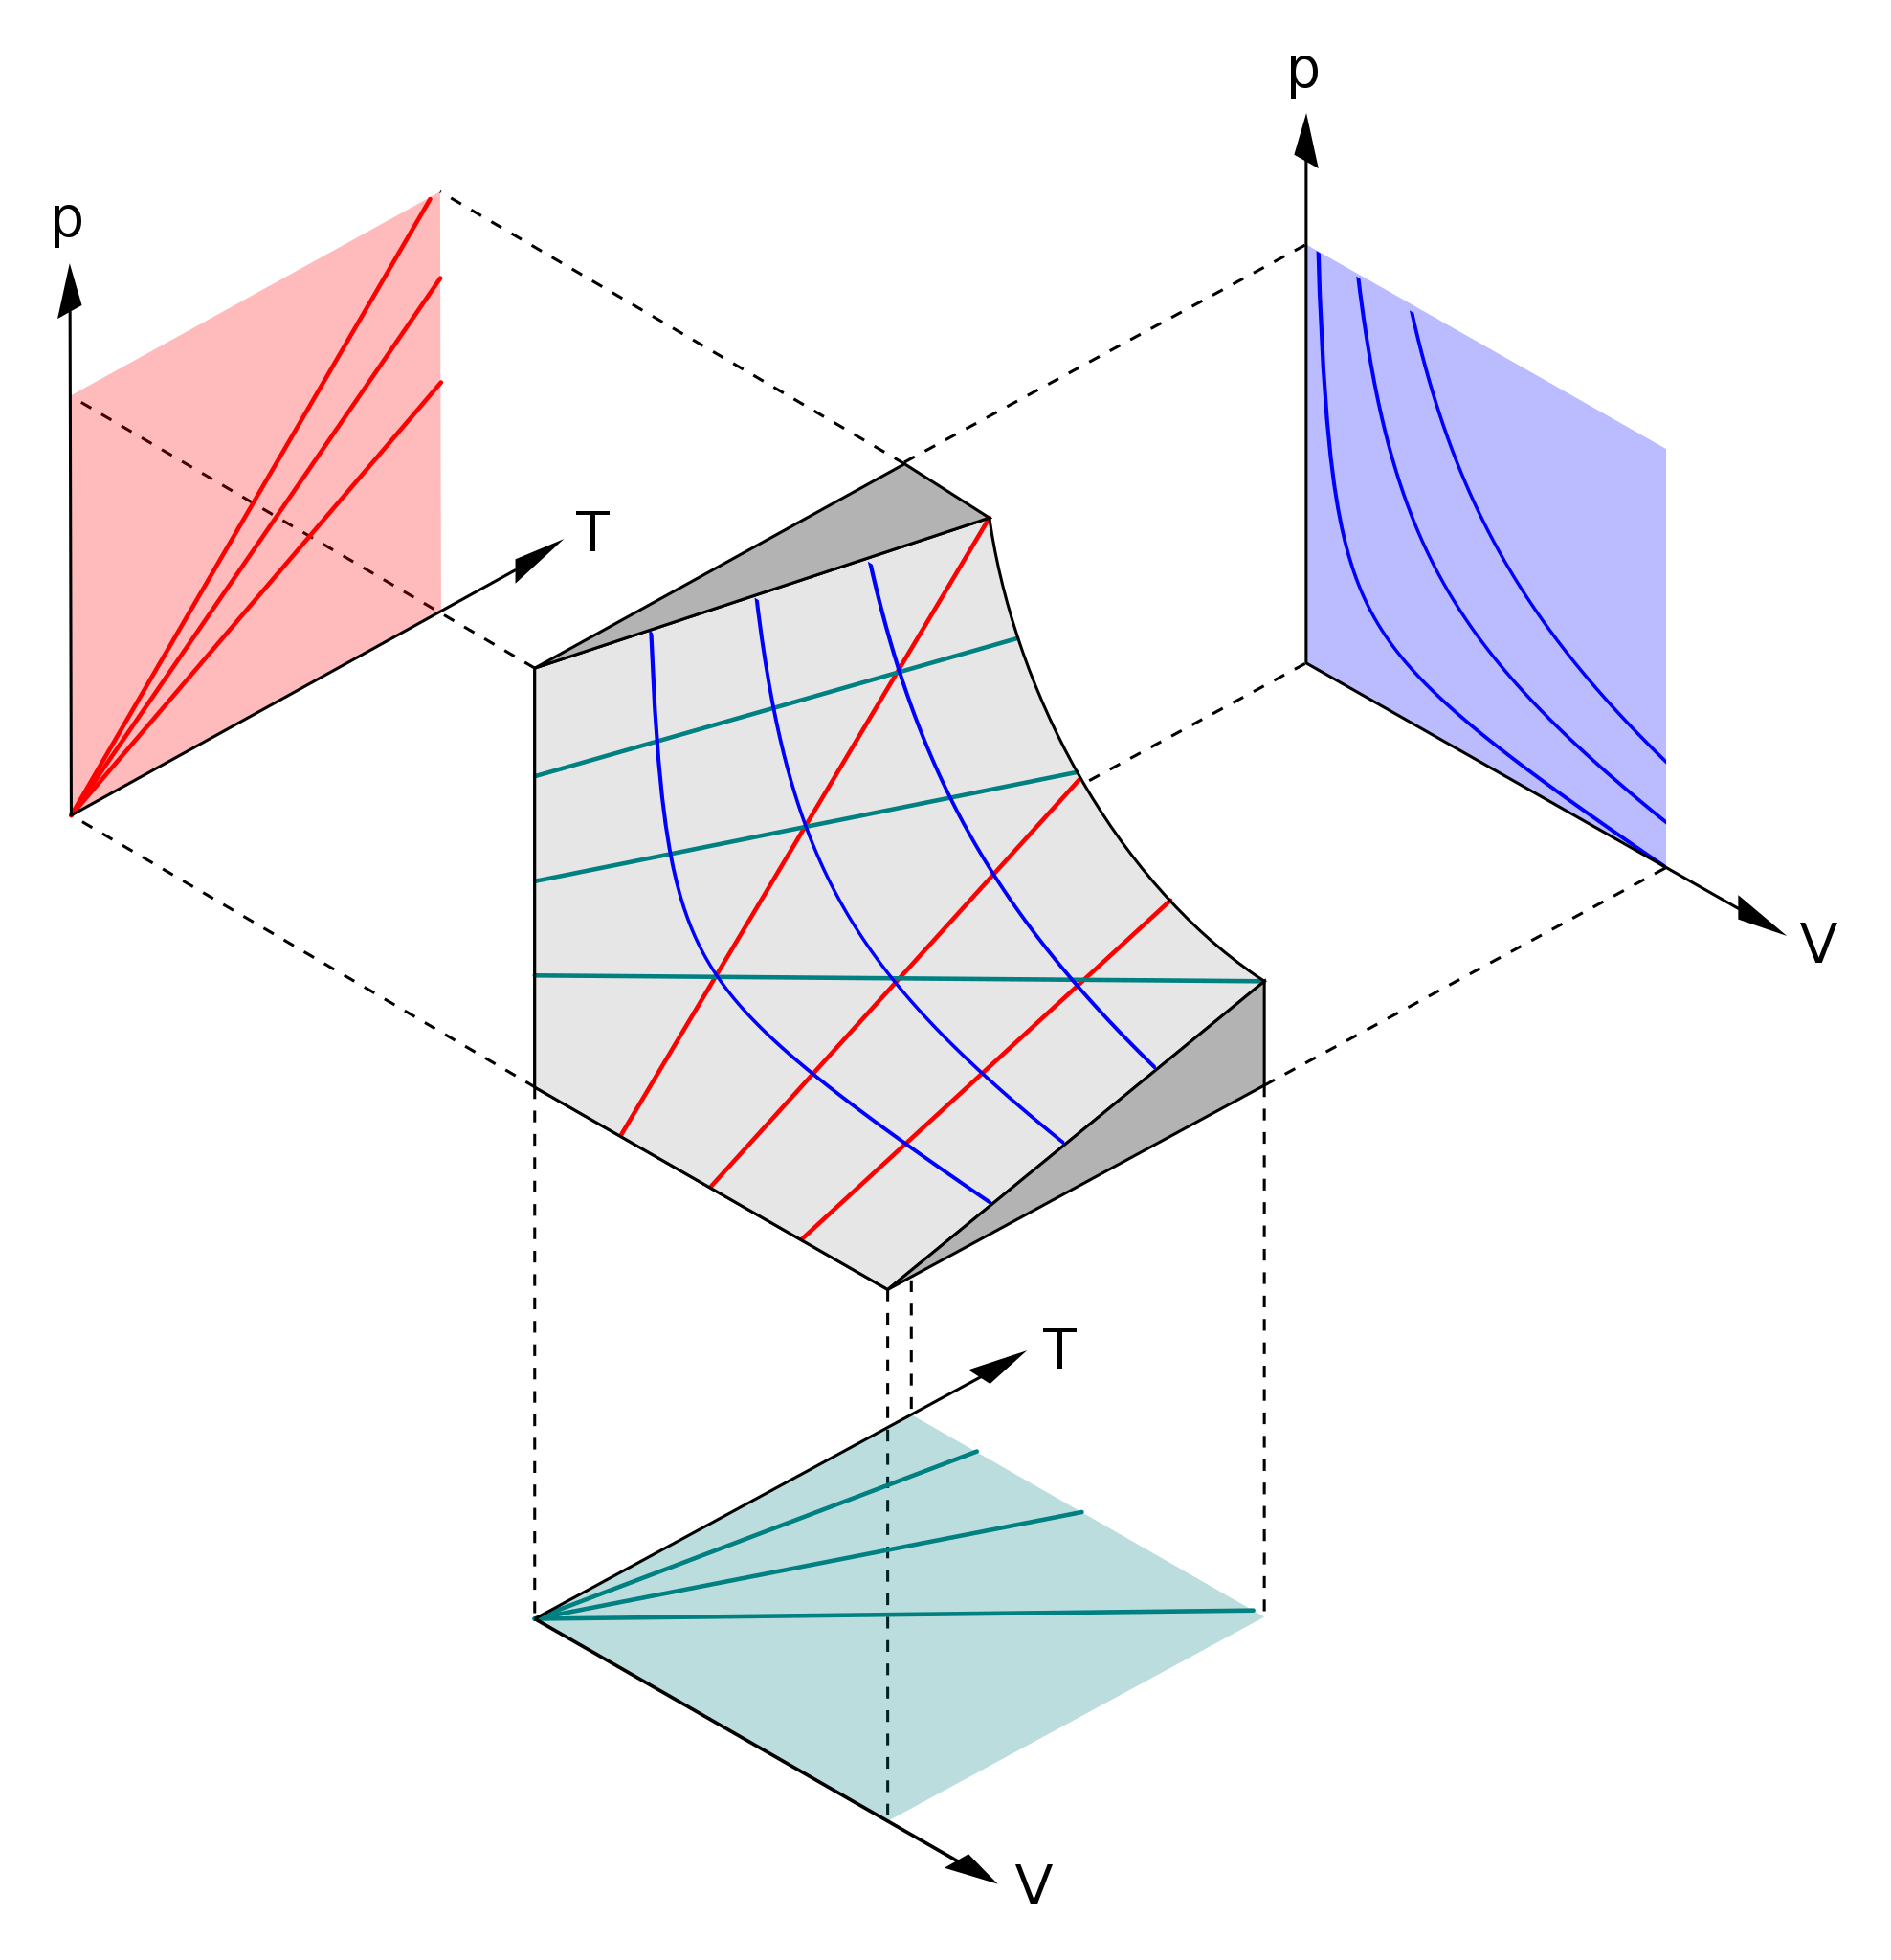
\includegraphics[width=14cm]{images/pVT-surface.png}
\end{figure}

\vocab{Mole} $n$: amount of substance that contains the same number of particles as the number of atoms in 0.012 kg (or 12 g) of carbon-12.

\vocab{Avogardo constant} $N_A$: number of particles in one mole of substance.
\[ N_A = \frac{N}{n} = 6.02 \times 10^{23} \: \unit{mol^{-1}} \]

\vocab{Boltzmann's constant}: gas constant per molecule.
\[ k_B = \frac{R}{N_A} = 1.38\times10^{-23} \: \unit{J.K^{-1}} \]

Rewriting the equation of state in \emph{number of molecules} gives us
\begin{equation}
pV=Nk_BT
\end{equation}

\vocab{Molar mass} of a substance $Mr$: mass of one mole of substance.
\[ Mr = \frac{m}{n} \]

\vocab{Molar volume} of a gas $V_m$: volume of one mole of gas.
\[ V_m = \frac{V}{n} \]
\pagebreak

\subsection{Kinetic theory of gases}
\textbf{Assumptions} of the kinetic theory of gases:
\begin{enumerate}
\item Gas consists of a very large number of particles.
\item Gas particles are in constant random motion and obey Newton's laws of motion.
\item No forces of attraction or repulsion between gas particles except during collision.
\item Gas particles behave as perfectly elastic, identical, hard spheres,
\item Total volume of the gas particles is negligible compared to volume of container.
\item Time duration of collision is negligible compared to time interval between collisions.
\end{enumerate}

Explain how molecular movement causes the pressure exerted by a gas.
\begin{itemize}
\item Gas molecules have rapid and random motion.
\item When they hit the walls of the container, they exert a force.
\item Pressure = Force/Area
\end{itemize}

We have the following relationship.
\begin{equation}
pV = \frac{1}{3}Nm\langle c^2 \rangle
\end{equation}

\deriv{See Appendix for the derivation.}

Related equations include
\[ pV=\frac{1}{3}Nm\langle c^2\rangle \iff \frac{1}{3}M\langle c^2\rangle \iff \frac{1}{3}nM_r\langle c^2\rangle \]

Using this, we can deduce the mean translational kinetic energy of one molecule.
\begin{equation}
\langle\text{KE}\rangle=\frac{1}{2}m\langle c^2\rangle = \frac{3}{2}k_BT
\end{equation}
This means that mean KE of a molecule of an ideal gas is \emph{proportional} to the thermodynamic temperature.

Thus total translational kinetic energy of $N$ molecules is given by
\begin{equation}
N\langle\text{KE}\rangle=\frac{3}{2}Nk_BT=\frac{3}{2}nRT
\end{equation}
\pagebreak

\subsection*{Problems}
\begin{prbm}
A resistance thermometer gives a resistance of 20 $\Omega$ when the temperature is known to be $-10$ \degree C. When the temperature is 110\degree C, the resistance thermometer has a resistance of 500 $\Omega$. What is the temperature when the resistance is 360 $\Omega$?
\end{prbm}
\begin{solution}
\[ \frac{\theta-(-10)}{110-(-10)}=\frac{360-20}{500-20} \implies \boxed{\theta=75\degree} \]
\end{solution}

\begin{prbm}
Two bulbs, $X$ of volume $100\:\unit{cm^3}$ and $Y$ of volume $50\:\unit{cm^3}$, are connected with a tube of negligible volume. A valve prevents gas to flow between the two bulbs. Initially bulb $X$ is filled with an ideal gas at 10\degree C to a pressure of $3\times10^5\:\unit{Pa}$. Bulb $Y$ is filled with the same ideal gas at 100\degree C to a pressure of $1\times10^5\:\unit{Pa}$. The valve is opened and the temperature of $X$ and $Y$ are maintained at their initial temperatures. Determine the new equilibrium pressure of the system.
\end{prbm}
\begin{solution}
Both bulbs exchange molecules until pressure is equal.

Total number of particles is conserved.
\begin{align*}
n_{X,i}+n_{Y,i} &= n_{X,f}+n_{Y,f} \\
\frac{P_{X,i}V_x}{T_X}+\frac{P_{Y,i}V_Y}{T_Y} &= \frac{P_fV_X}{T_X}+\frac{P_fV_Y}{T_Y}
\end{align*}
$\therefore\quad \boxed{P_f=2.45 \times 10^5\:\unit{Pa}}$
\end{solution}
\pagebreak